View demo code of this section: \democode{02}{2.4}

The quantum circuit is a graphical representation of the sequence of quantum gates applied to qubits in a quantum computation or quantum algorithm. Similar to classical digital circuits made up of logic gates that manipulate classical bits, quantum circuits are composed of quantum gates that manipulate quantum bits or qubits.

\subsubsection{Construct a quantum circuit}
In \MindQuantum we use \Circuit to represent quantum circuit:

\begin{lstlisting}
from mindquantum.core.circuit import Circuit
circ = Circuit()
\end{lstlisting}

There are several basic operations for adding a quantum gate into \Circuit
\begin{itemize}
    \item +=: use '+=' to add a quantum gate to the circuit.
    \item Circuit.x: add an X gate to the circuit.
    \item list: directly construct a quantum gate with gate list
\end{itemize}
\begin{lstlisting}
from mindquantum.core.gates import H, Y, X, Z
circ = Circuit([X.on(0), Y.on(1)])
circ += H.on(0)
circ += Y.on(1, 0)
circ.x(1, 0)
circ.z(2, [0, 1])
\end{lstlisting}

\subsubsection{Display a quantum circuit}
SVG(Scalable Vector Graphics) is based on the XML markup language and is used to describe vector graphics in two dimensions. \MindQuantum provides a function to export quantum circuit to SVG format.
\begin{lstlisting}
circ.svg().to_file(filename='circuit.svg')
\end{lstlisting}
\begin{figure}[h]
    \begin{center}
        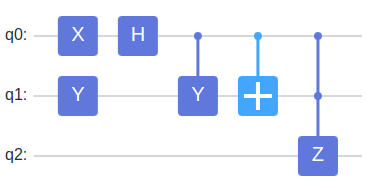
\includegraphics[width=0.9\linewidth]{images/2_4_circuit.png}
    \end{center}
    \caption{Quantum Circuit.}
\end{figure}
Please note that if you are in jupyter notebook environment, you can directly get svg image by \code{circ.svg()}.


\subsubsection{Common interfaces}

Quantum Circuit is the basic element of quantum algorithm, \MindQuantum provide a lot of useful method for \Circuit.

\begin{itemize}
    \item \propnqubits: get the number of qubit of quantum circuit.
    \item \propparamsname: get the params of circuit.
    \item \prophasmeasuregate: get whether to be measured.
    \item \methodmatrix: get the circuit matrix.
    \item \methodgetqs: get the final quantum state.
    \item \methodsummary: get information about the current circuit, including the number of blocks, gates, gates without parameters, gates with parameters and parameters.
\end{itemize}

\subsubsection{Advanced operator on circuit}

Constructing a large size quantum circuit is always not a straightforward thing for user. Here in \MindQuantum, we can use some pre-defined method to manipulate your \Circuit very easily. For example the origin quantum circuit is:

\begin{lstlisting}
from mindquantum.core.circuit import *

circ = Circuit().h(0).rx('a', 2, 0)
\end{lstlisting}

\begin{figure}[H]
    \begin{center}
        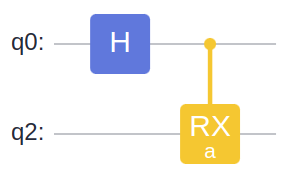
\includegraphics[width=0.6\linewidth]{images/2_4_ori_circ.png}
    \end{center}
    \caption{Quantum Circuit need to manipulate.}
\end{figure}
We now show how to manipulate on this quantum circuit:


\begin{enumerate}
    \item \methodcompress{circ} : compress all qubit to first $n$ qubits.\par
          \begin{minipage}{\linewidth}
              \centering
              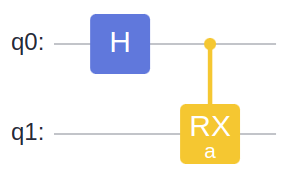
\includegraphics[width=0.6\linewidth]{images/2_4_compress_circ.png}
          \end{minipage}
    \item \methodcontrol{circ}{1} : add control qubits on this circuit\par
          \begin{minipage}{\linewidth}
              \centering
              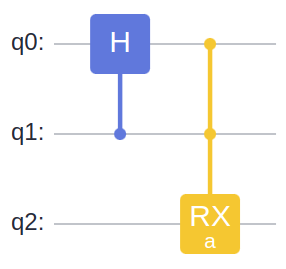
\includegraphics[width=0.6\linewidth]{images/2_4_ctrl_circ.png}
          \end{minipage}
    \item \methoddagger{circ} : get hermitian conjugate version\par
          \begin{minipage}{\linewidth}
              \centering
              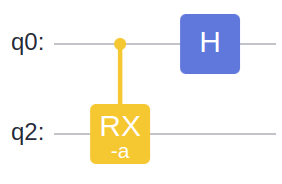
\includegraphics[width=0.6\linewidth]{images/2_4_dagger_circ.png}
          \end{minipage}
    \item \methodapply{circ}{[2, 1]} : apply circuit to other qubits\par
          \begin{minipage}{\linewidth}
              \centering
              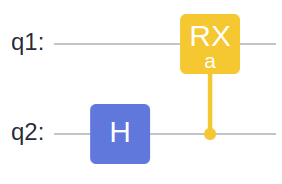
\includegraphics[width=0.6\linewidth]{images/2_4_apply_circ.png}
          \end{minipage}
    \item \methodreverse{circ} : reverse the qubit order in circuit\par
          \begin{minipage}{\linewidth}
              \centering
              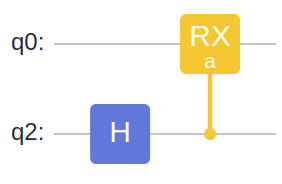
\includegraphics[width=0.6\linewidth]{images/2_4_reverse_circ.png}
          \end{minipage}
    \item \methodshift{circ}{2} : shift the qubit range with given step\par
          \begin{minipage}{\linewidth}
              \centering
              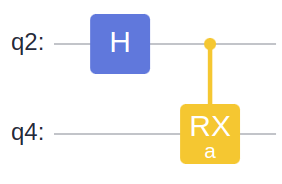
\includegraphics[width=0.6\linewidth]{images/2_4_shift_circ.png}
          \end{minipage}
\end{enumerate}
